% intro
\section{}

\begin{frame}
	\frametitle{Weitere Bibliografie}
	[7] Logo retrieval with a contrario visual query expansion [Alexis2009]\newline
	[8] Scalable mining of small visual objects [Alexis2012]\newline
	[9] Scalable Triangulation-based Logo Recognition [Kalantidis2011]\newline
	[10] Scalable logo recognition in real-world images [Romberg2011]\newline
	[11] Deep learning for logo recognition [Bianco2017]\newline
	[12] Deep Learning Logo Detection with Data Expansion by Synthesising Context [Su2016]
\end{frame}

\begin{frame}
	\center\Huge Anhang
\end{frame}

\begin{frame}
	\frametitle{Siam-Logos Test Phase}
	\begin{figure}
	        \centering
        		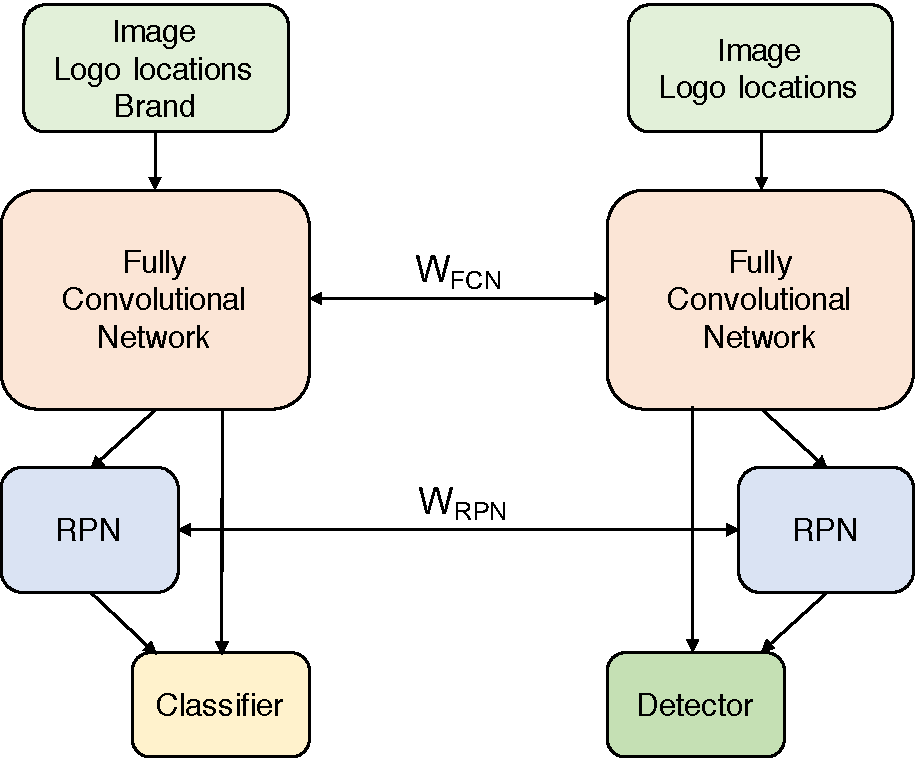
\includegraphics[height=60mm]{sol5_arch_train} 
	\end{figure}
\end{frame}

\begin{frame}
	\frametitle{�hnlichkeitsscores}
	\begin{figure}
	        \centering
        		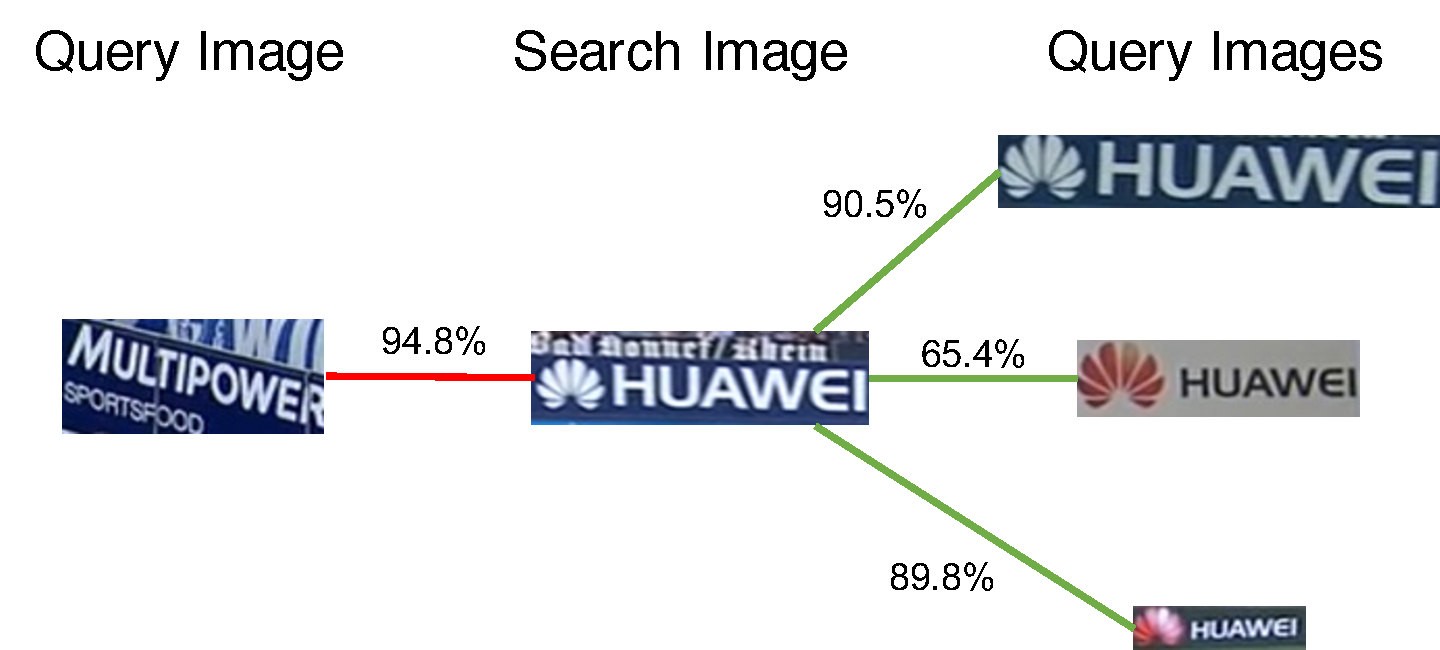
\includegraphics[height=50mm]{cosdistance} 
	\end{figure}
\end{frame}

\begin{frame}
\frametitle{Evaluation}
	\heading{Logo Detektion}
	\begin{figure}
	        \centering
       		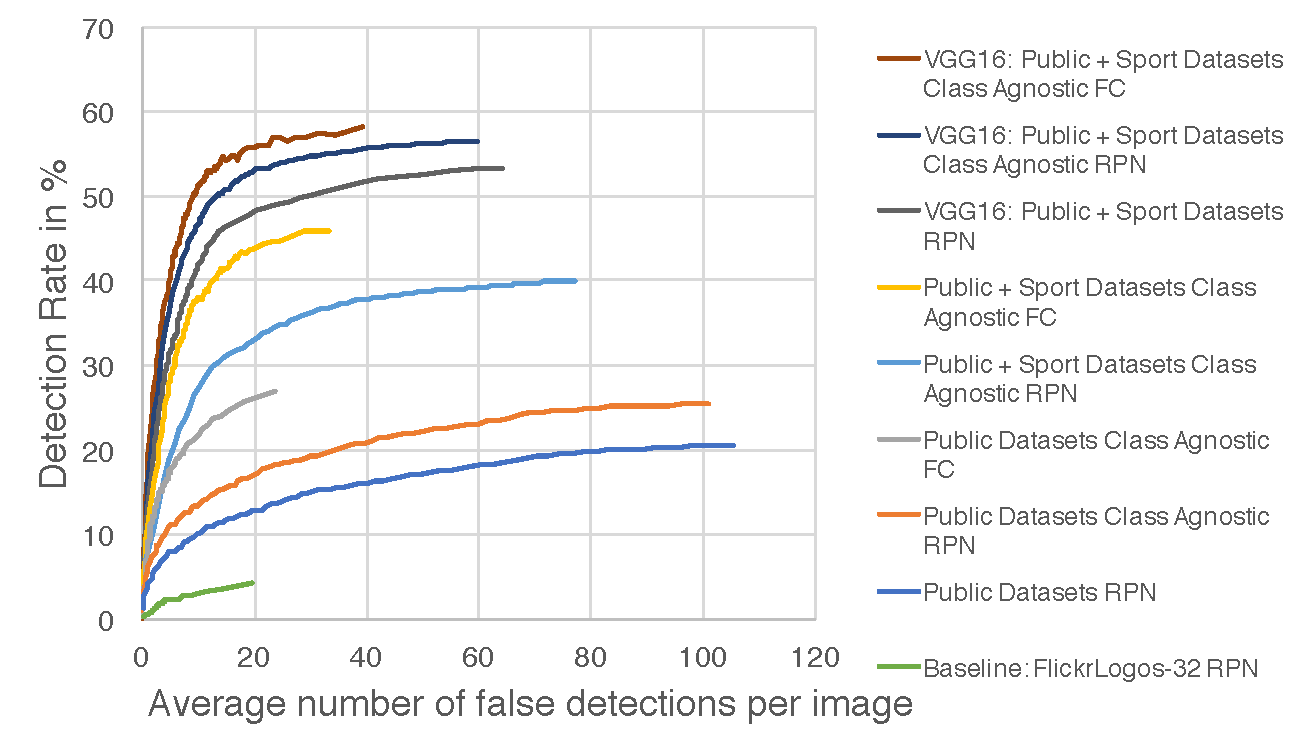
\includegraphics[height=55mm]{detection_full} 
	\end{figure}
\end{frame}

\begin{frame}
	\frametitle{Evaluation}
	\heading{Fast-Logos, Fast	\&Faster-Logos vs. Baseline}
	\begin{figure}
	        \centering
       		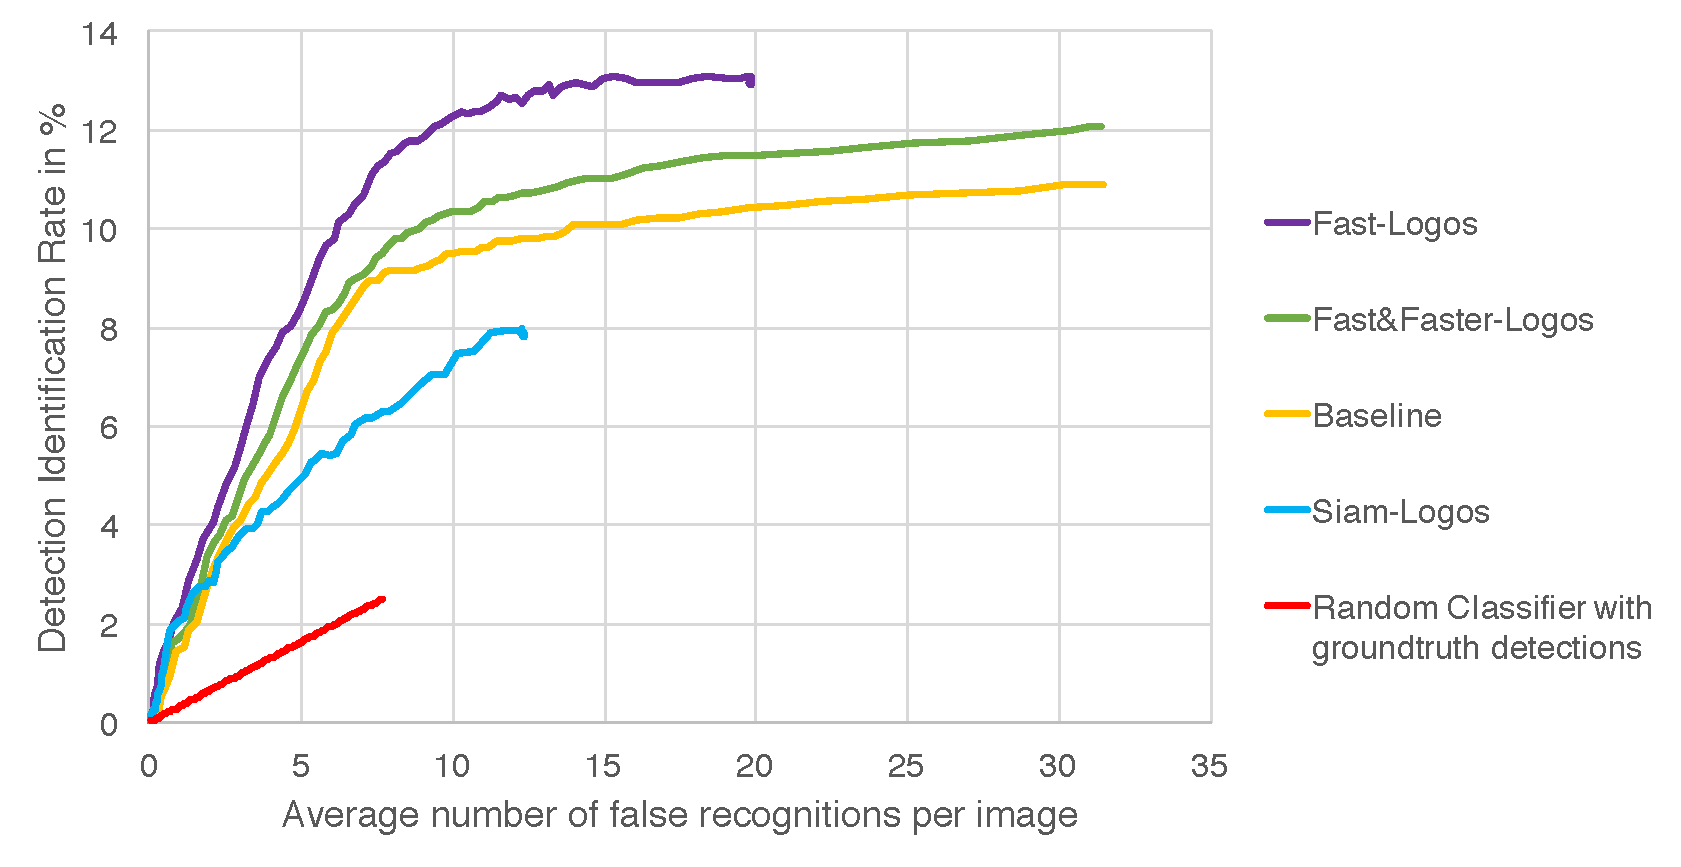
\includegraphics[height=55mm]{eval1} 
	\end{figure}
\end{frame}

\begin{frame}
	\frametitle{Evaluation}
	\heading{R-CNN-Logos vs. Baseline}
	\begin{figure}
	        \centering
       		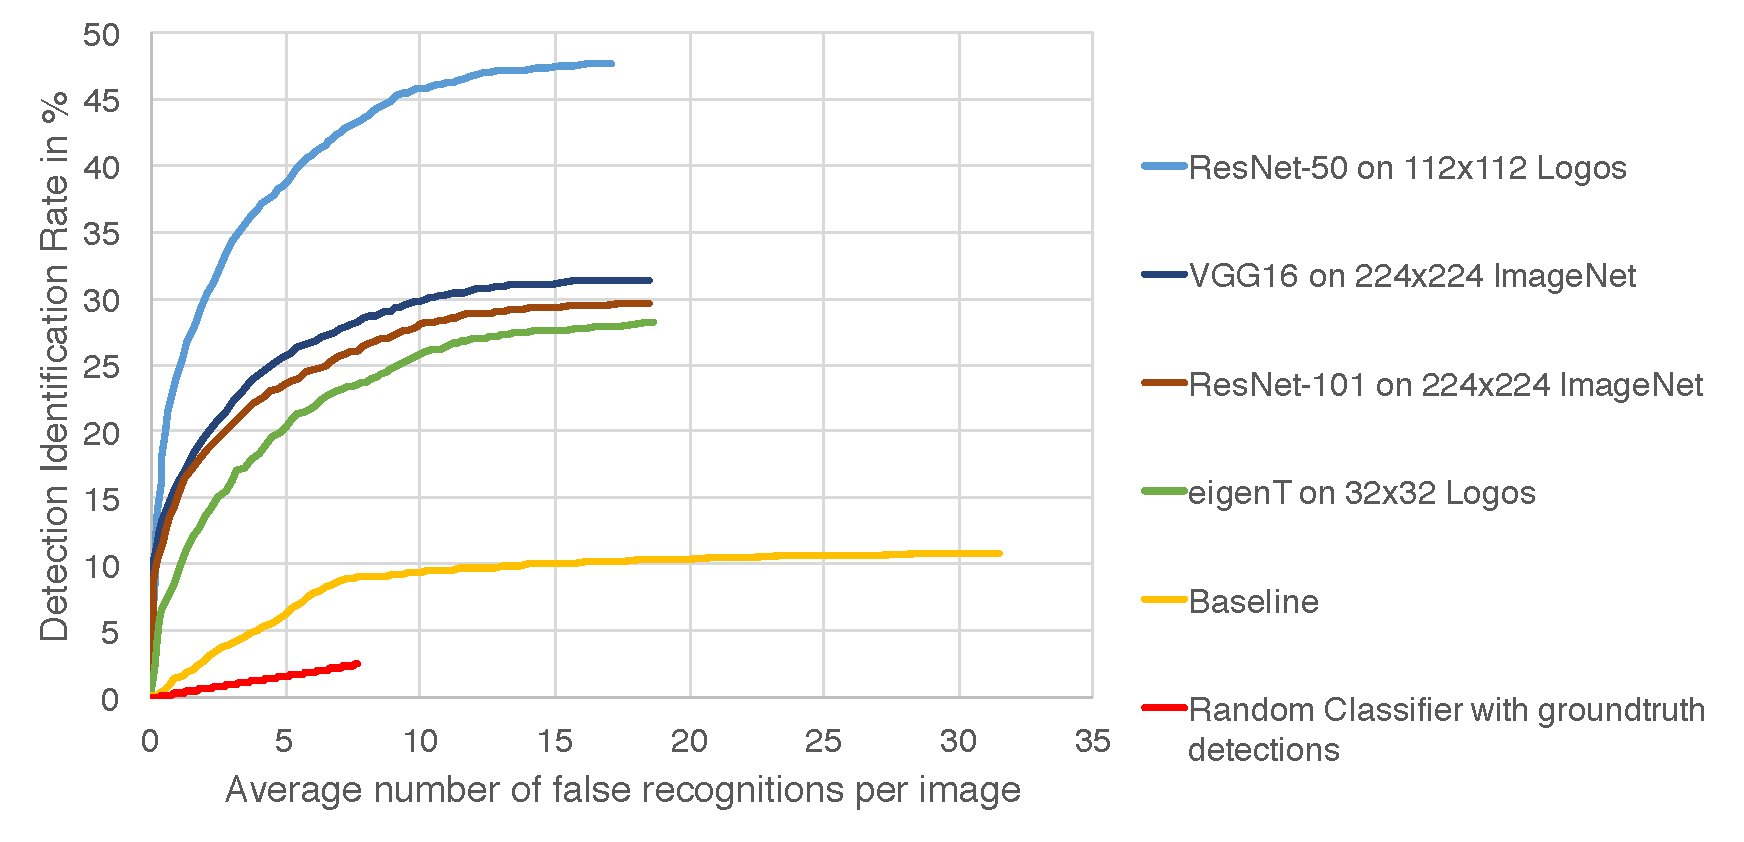
\includegraphics[height=55mm]{eval2} 
	\end{figure}
\end{frame}

\begin{frame}
	\frametitle{Evaluation}
	\heading{Verarbeitungszeit pro Bilder und beste DIR Werte}
	\begin{figure}
	        \centering
       		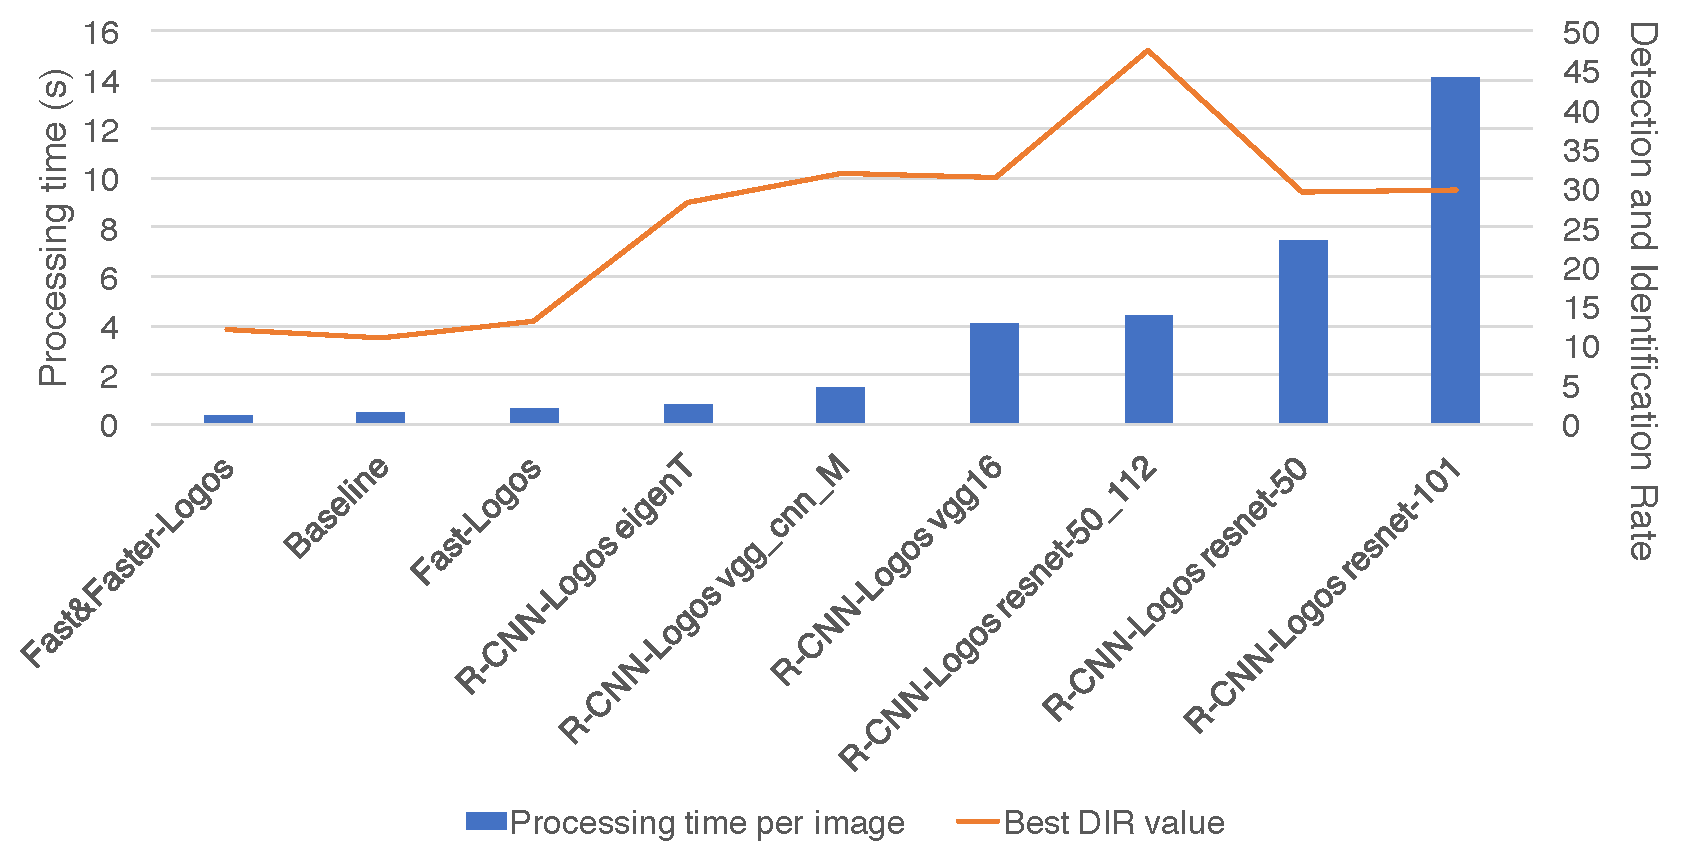
\includegraphics[height=55mm]{timeeval} 
	\end{figure}
\end{frame}

\begin{frame}
	\frametitle{Evaluation}
	\heading{Performance von Klassen, die in dem Training-Set vorkommen}
	\begin{figure}
	        \centering
       		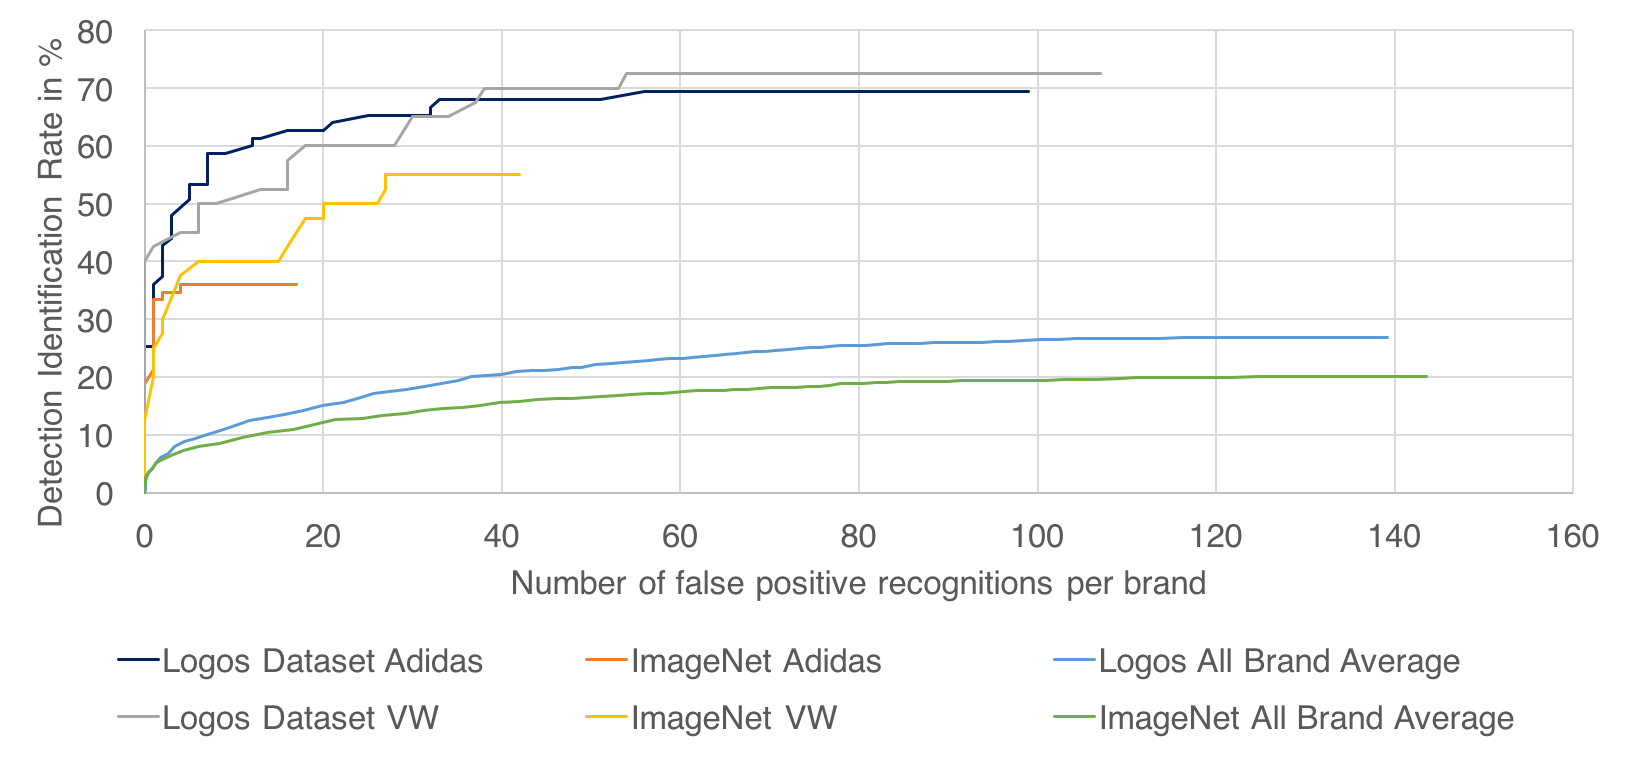
\includegraphics[height=50mm]{commonbrandseffect} 
	\end{figure}
\end{frame}

\begin{frame}
	\frametitle{Evaluation}
	\heading{Logo Vergleich}
	\begin{figure}
	        \centering
       		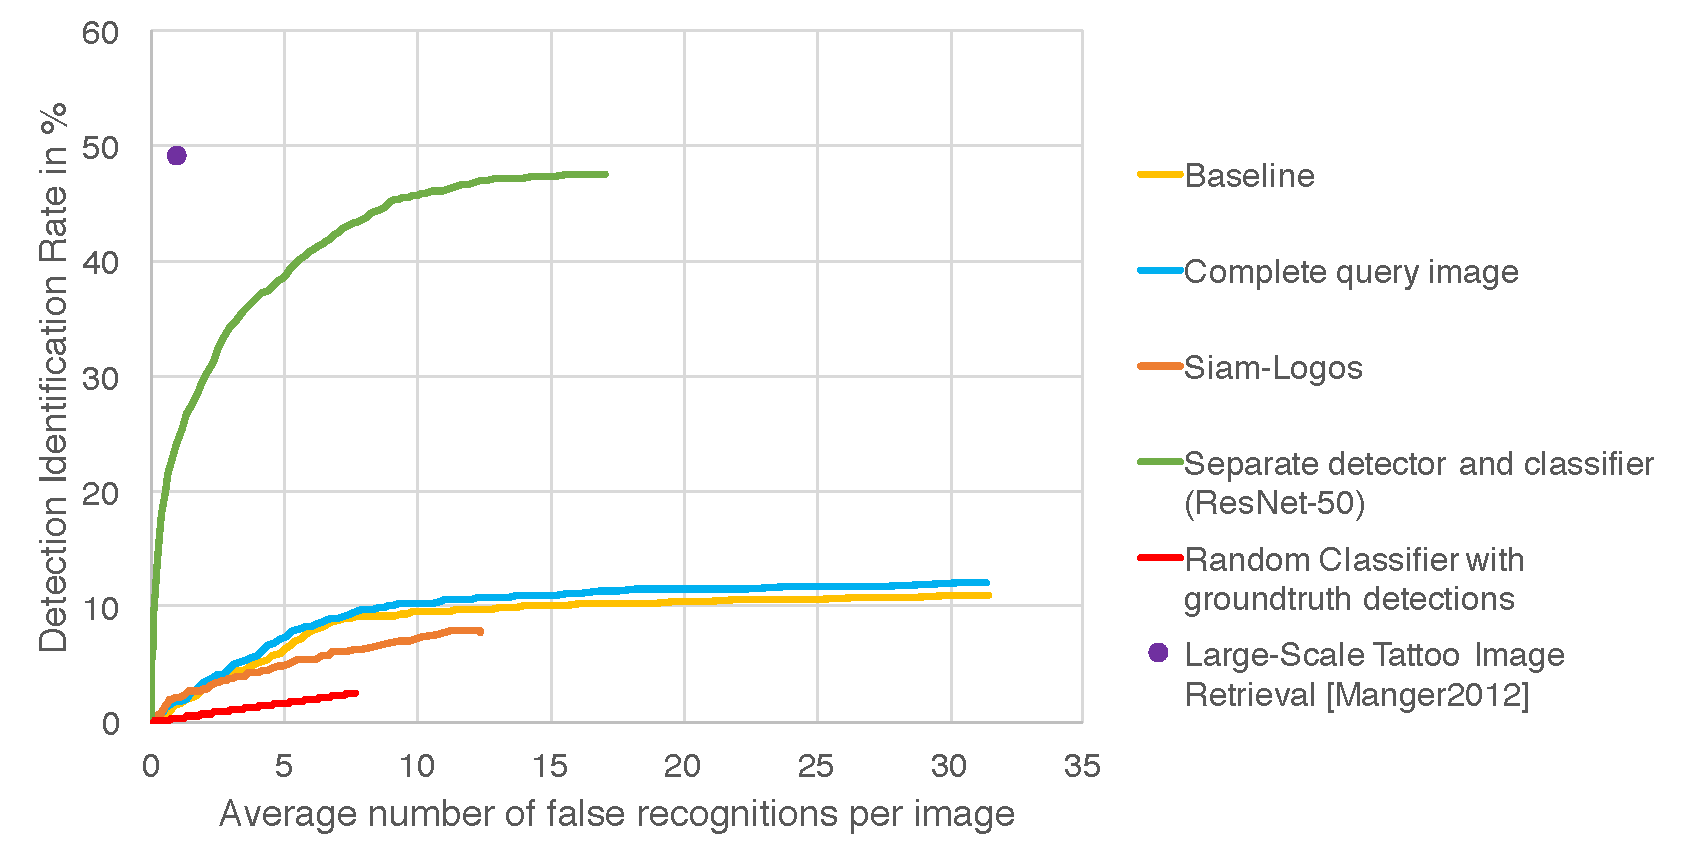
\includegraphics[height=50mm]{clsevalfull} 
	\end{figure}
\end{frame}